\section{Vorlesung 16.12.2016}

Metrik:
\begin{enumerate}
	\item $d_{uu}=0$
	\item $d_{uv}=0 \Rightarrow u=v$
	\item $d_{uv}=d_{vu}$
	\item $d_{uv} + d_{vw} \geq d_{uw}$ (Dreiecksungleichung)
\end{enumerate}

Pseudometrik: -,1,2,3\\
Metrik: 0,1,2,3\\
Distanzfunktion: 1,2\\

\fcolorbox{red}{white}{\parbox{\linewidth}{\textbf{4-Punkte-Bedingung:}\\
Eine Distanzfunktion d ist eine additive (Baum) Metrik wenn je vier Punkte so geordnet werden können, daß:\\
$d_{xy} + d_{uv} \leq d_{xu} + d_{yv} = d_{xv} + d_{yu} \Leftrightarrow \forall$x,y,u,v gilt:\\
$d_{xy} + d_{uv} \leq max\{d_{xu} + d_{yv}, d_{xv} + d_{yu}\}$}}
\\\\\\
\fcolorbox{red}{white}{\parbox{\linewidth}{\textbf{Isolationsindex:}\\
$l(e)=\alpha(A|B)=max(0, \displaystyle\min_{\substack{x,y \in A \\ u,v \in B}} \frac{1}{2}[max\{d_{xu} + d_{yv}, d_{xv} + d_{yu}\} - (d_{xy} + d_{uv})])$\\
=Länge der Baumkante, die A,B trennt oder $\leq$ 0 wenn $A|B$ keine Teilbäume bestimmt.}}\\\\
Wenn d eine additive Distanzfunktion:
\begin{itemize}
	\item $\alpha (A|B)\geq 0$
	\item $A|B$ entspricht einer Kante im Baum $\Leftrightarrow$ $\alpha (A|B) > 0$
\end{itemize}

Splitpseudometrik:
\begin{equation}
	\delta_{A|B}(x,y)= \begin{cases}
		1:x\in A, y \in B\\
		1:x\in B, y \in A\\
		0:x,y \in A\\
		0:x,y \in B\\
	\end{cases}
\end{equation}

x,y durch $A|B$ getrennt $\Leftrightarrow \delta_{A|B}(x,y)=1$\\
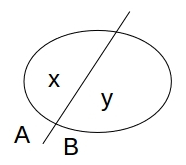
\includegraphics[width=0.2\textwidth]{lectures/161216/pix/1.jpg}\\

\fcolorbox{red}{white}{\parbox{\linewidth}{
$d_T(x,y)=\displaystyle\sum_{(A|B) \in \Sigma (T)} \alpha(A|B) \cdot \delta_{A|B}(x,y)$}}\\\\

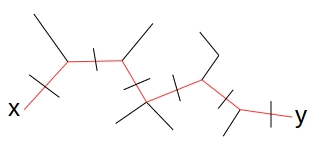
\includegraphics[width=0.7\textwidth]{lectures/161216/pix/2.jpg}\\

Genau die splits entlang des Pfades von x und y trennen x,y
\\\\
\textbf{Splits $\Sigma(T) \rightarrow$ Baum}\\
wir wissen $\Sigma(T)$ ist kompatible\\
$A|B,C|D \in \Sigma(T)$ dann mindestens einer der vier Durchschnitte:\\ $A \cap C, A \cap D, B \cap C, B \cap D$ leer\\
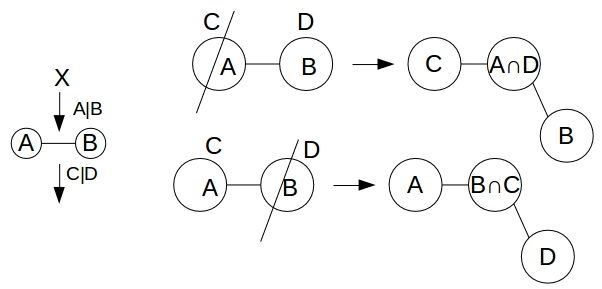
\includegraphics[width=0.7\textwidth]{lectures/161216/pix/3.jpg}\\
jeder split-Teil \underline{GENAU} eine der Mengen\\\\
\textbf{Frage:} Wie können Isolationsindizes, schnell und und alle Möglichkeiten durchzuprobieren, erzeugt werden?\\
Lösung: effiziente Berechnung von $\alpha(A|B)>0$\\
Idee: erweitere X schrittweise\\
$|A|,|B|=1$\\
$X' \leftarrow X \cup \{w\}$\\
$A\cup B=X$\\
in $X':$\\
- \hspace{10pt}$X|\{w\}$\\
- \hspace{10pt}$A\cup \{w\}|B$\\
- \hspace{10pt}$B\cup \{w\}|A$\\
\\\\
$\beta_{xy|uv}:=\frac{1}{2}max\{d_{xu} + d_{yv}, d_{xv} + d_{yu}\} - (d_{xy} + d_{uv})$\\
erster Fall:\\
$\alpha(\{x\}|X)=\displaystyle\min_{u,v \in X}\beta_{ww|uv}=\displaystyle\min_{u,v \in X} \frac{1}{2}(d_{wu} + d_{wv} - d_{uv})$\\
zweiter Fall:\\
$\alpha(A|B)=\displaystyle\min_{\substack{x,y \in A \\ u,v \in B}}\beta_{xy|uv}$\\

$\alpha(A\cup\{w\}|B)=\min \{ \displaystyle\min_{\substack{x,y \in A \\ u,v \in B}} \beta_{xy|uv}, \displaystyle\min_{\substack{y \in A \\ u,v \in B}} \beta_{yw|uv}, \displaystyle\min_{\substack{x \in A \\ u,v \in B}} \beta_{xw|uv} \}$
\\\\
$\Rightarrow \alpha(A \cup \{w\}|B) \leq \alpha(A|B)$\\
Also: wenn $\alpha(A|B) \leq 0 \Rightarrow \alpha(A \cup \{w\}|B)$ auch $\leq0$\\ 
$\Rightarrow$ nur Splits auf X mit $\alpha(A|B)>0$ müssen erwartet werden\\
Wenn d additiv $\Rightarrow$ Baum $\Rightarrow$ splits$\Sigma(T)$ kompatibel $\Rightarrow$ es gibt nicht mehr als $2|X|$ splits\\
$\Rightarrow$Die Isolationsindizes aller Splits mit $\alpha(A|B)>0$ können in $\mathcal{O}(|x|^5)$ berechnet werden:\\
$|x|$ Erweiterungsschritte für $\mathcal{O}(|x|)$ splits mit Aufwand $\mathcal{O}(|x|^3)$\\\\

\fcolorbox{red}{white}{\parbox{\linewidth}{
\underline{Theorem:}[Bandelt,Dress]\\
Sei d eine Peusometrik auf X. Dann gibt es eine Pseudometrik $d^0$ auf X sodaß\\
$d(x,y)=\displaystyle \sum_{A|B}\underbrace{\alpha(A|B)}_{*} \cdot \delta_{A|B}(x,y) + d^0(x,y)$\\
* $\alpha(A|B)=0$ wenn $\displaystyle\min_{\substack{x,y \in A \\ u,v \in B}}\beta_{xy|uv}<0$}}
\\\\
außerdem gilt:
$\Sigma(d)=\{(A|B)\}\\alpha(A|B)>0$ hat höchstens $\mathcal{O}(|x|^2)$ Elemente\\
alle $\alpha(A|B)>0$ können in $\mathcal{O}(|x|^6)$ Elemente berechnet werden.\\
\begin{itemize}
	\item d additiv $\Rightarrow d^0=0$
	\item $d^0$ heißt split-primer
	\item d heißt total zerlegbar wenn $d^0=0$
\end{itemize}

\textbf{allgemeine Pseudometrik auf 4 Punkten}\\
Anzahl unabhängigen Distanzen: 6\\
Baum mit 4 Blättern: 5
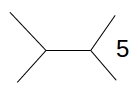
\includegraphics[width=0.15\textwidth]{lectures/161216/pix/4.jpg}\\
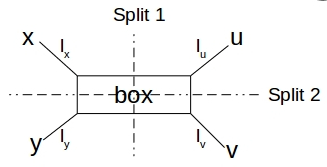
\includegraphics[width=0.75\textwidth]{lectures/161216/pix/5.jpg}\\
$d_{xu} + d_{xy} - d_{duy}$\\
$(l_x+a+l_u)+(l_x+b+l_y)-l_u-a-b-l_y=2l_x$\\
$l_x=\frac{1}{2}[\underbrace{d_{xu}+d_{xy}-d_{uy}}_{\geq 0 (Dreiecksungleichung)}]$\\\\
Split 1:\\
$d_{xv}+d_{yu}-(d_{xy}+d_{uv})$=\\
$l_x+a+b+l_v$\\
$+l_y+a+b+l_u$\\
$-l_x-b-l_y$\\
$-l_u-b-l_v=2a$\\\\
Split 2:\\
$d_{xu}+d_{yv}-(d_{xy}+d_{uv})$=\\
$l_x+a+l_u$\\
$+l_y+a+l_v$\\
$-l_x-b-l_y$\\
$-l_y-b-l_u=2(a-b) \leq 2a$\\\\

$\alpha(\{xy\}|\{uv\})=a$\\
$\alpha(\{xu\}|\{yv\})=b$\\
Baum $\Rightarrow$ b=0\\\\

\textbf{Messung der Baumartigkeit:}\\
$B:=\frac{1}{\binom{n}{4}} \displaystyle\sum_{\substack{i<j<k<l \\ i,j,k,l \in X}} \frac{b_{ijkl}}{a_{ijkl} + b_{ijkl}}$\\
Mittelwerte von in der Box\\
B $\approx$ Baumartig\\
B $\approx \frac{1}{2}$ völlig verrauscht, netzwerk-artig\\

\textbf{Travelling sales person problem (TSP)}\\
geschlossene Tour Voraussetzung\\
$|X|>1$ (Anzahl der Städte größer 1)\\
Metrik d auf X gegeben\\
Tour: Permutation von X:$\pi$\\
$L(\pi)=\displaystyle\sum_{i=1}^{|X|}d_{\pi(i-1)\pi(i)}$ (lesen als indices modulo $|X|$)
\\\\
\fcolorbox{red}{white}{\parbox{\linewidth}{
Definition Mastertour:\\
Einschränkung von $\pi$ auf $X'\subseteq X$ löst das TSP auf X\\\\
Wenn d eine additive Metrik (Baum) ist dann existiert eine Mastertour (optimale Lösung) die genau ein Mal um den Baum herum führt.}}\\
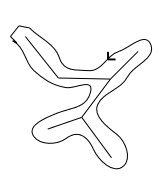
\includegraphics[width=0.2\textwidth]{lectures/161216/pix/6.jpg}\\

\fcolorbox{red}{white}{\parbox{\linewidth}{
Eine Metrik hat die KALMANSON-Eigenschaft, wenn man X so ordnen kann, daß\\
$d_{ij}+d_{kl}\leq d_{ik} + d_{jl} \forall i<j<k<l$\\
und\\
$d_{il}+d_{jk}\leq d_{ik} + d_{jl} \forall i<j<k<l$}}\\
$\rightarrow$ für jedes Quadrupel tauchen höchstens die Splits ij$|$kl, il$|$jk auf\\
d ist Kalmanson $\Leftrightarrow$ das TSP mit Distanz d einen Mastertour hat\\
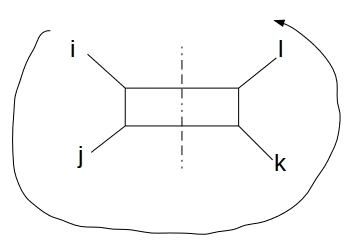
\includegraphics[width=0.5\textwidth]{lectures/161216/pix/7.jpg}\\
Wenn d Kalmanson ist (zirkulär zerlegbar) $\Rightarrow$ d splitzerlegbar (planar darstellbar)\\
$\nLeftarrow$ (Umkehr falsch)\\

$d=\underbrace{\displaystyle\sum_{A|B}\alpha(A|B) \cdot \delta_{A|B}}_{fast\ immer\ Kalmanson} + \underbrace{\delta^0}_{\substack{Rauschen \\ (split\ Primaeranteil)}}$\\\\\\
Anteil der Distanz ohne phylogenetische Information:\\
$\frac{\displaystyle\sum_{x\neq y} \delta^0(x,y)}{\displaystyle\sum_{x\neq y} \delta(x,y)}$\\
(Maß für die Größe des Rauschens $\rightarrow$ keine phylogenetische Information)